\bookchapter{Sensors}\label{ch:hw4}

\section*{Explanation}
A robot knows nothing about the world except what its sensors measure, and every sensor is imperfect: noisy, delayed, biased, limited in range. Most of the engineering of a walking robot is about getting a good picture out of bad measurements. This chapter explains the sensors of a humanoid soccer robot (joint encoders, an IMU, cameras, force sensors), the vocabulary to describe their quality, and the first and most useful trick to combine them: sensor fusion.

\section*{How to describe a sensor}
\begin{center}
\renewcommand{\arraystretch}{1.25}
\begin{tabular}{p{3.0cm}p{10.0cm}}
\textbf{Property} & \textbf{Meaning}\\ \hline
Range & smallest and largest value that can be measured (a gyroscope: $\pm2000^\circ$/s)\\
Resolution & smallest change that can be told apart; for digital sensors the step of the ADC (Chapter~\ref{ch:hw3}), e.g.\ $4000^\circ/\text{s}/2^{16}=0.061^\circ/\text{s}$ per bit\\
Accuracy & how close the average measurement is to the true value (small \emph{bias})\\
Precision & how close repeated measurements are to each other (small \emph{noise})\\
Sample rate & measurements per second (Hz)\\
Latency & time between the event and the arrival of the value in your program\\
Drift & slow change of the error over time or with temperature\\
\end{tabular}
\end{center}
Accuracy and precision are different (Figure~\ref{fig:hw4_acc}). A precise but inaccurate sensor has a constant error that you can \emph{calibrate} away (measure a known value, subtract the offset); a noisy but accurate sensor is improved by averaging.
\begin{center}
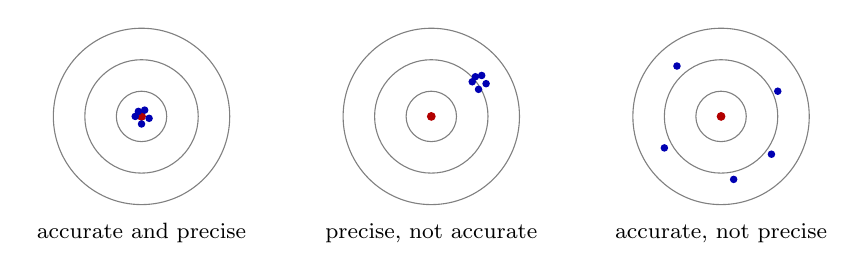
\begin{tikzpicture}[scale=0.8]
  \foreach \x/\lab/\dx/\dy in {0/{accurate and precise}/0.0/0.0, 4.6/{precise, not accurate}/0.75/0.55, 9.2/{accurate, not precise}/0/0}{
    \begin{scope}[xshift=\x cm]
      \foreach \r in {0.4,0.9,1.4}{\draw[gray] (0,0) circle (\r);}
      \fill[red!70!black] (0,0) circle (0.07);
      \node[font=\footnotesize] at (0,-1.85) {\lab};
    \end{scope}}
  \foreach \px/\py in {0.05/0.1,-0.1/0.0,0.0/-0.12,0.12/-0.03,-0.05/0.08}{\fill[blue!70!black] (\px,\py) circle (0.06);}
  \foreach \px/\py in {0.05/0.1,-0.1/0.0,0.0/-0.12,0.12/-0.03,-0.05/0.08}{\fill[blue!70!black] ({4.6+0.75+\px},{0.55+\py}) circle (0.06);}
  \foreach \px/\py in {0.9/0.4,-0.7/0.8,0.2/-1.0,-0.9/-0.5,0.8/-0.6}{\fill[blue!70!black] ({9.2+\px},\py) circle (0.06);}
\end{tikzpicture}
\captionof{figure}{Measurements (blue) around the true value (red centre). Bias is the offset of the cluster, noise its spread.}\label{fig:hw4_acc}
\end{center}
\textbf{Sampling.} A sensor measures at discrete times. If a signal changes faster than half the sample rate (the \textbf{Nyquist frequency}), the samples show a false, slower signal: \textbf{aliasing}. A vibration of $90$\,Hz sampled at $100$\,Hz appears as a $10$\,Hz oscillation. Therefore: sample at least twice as fast as the fastest thing you care about (in practice five to ten times), and filter the signal \emph{before} sampling (every good sensor chip has such a filter, whose cut-off you configure).

\section*{Proprioception: knowing the own body}
\subsection*{Encoders}
An \textbf{encoder} measures the angle of a shaft. An \emph{incremental} encoder produces pulses when the shaft turns; two tracks A and B, shifted by a quarter period, give the \textbf{quadrature} signal that also tells the direction (Figure~\ref{fig:hw4_quad}): when A rises while B is low the shaft turns forward, otherwise backward. Counting all four edges per period gives $4\times$ the resolution: $1024$ lines yield $4096$ counts per turn, i.e.\ $0.088^\circ$ per count. An \emph{absolute} encoder (magnetic or optical) reports the angle within one turn directly, also right after power-up; the joints of modern robots use magnetic absolute encoders with $12$ to $19$ bit resolution. Encoder count and gear ratio give the angle at the \emph{output} of the gearbox (Chapter~\ref{ch:hw6}); the backlash of the gears is not seen by an encoder on the motor side.
\begin{center}
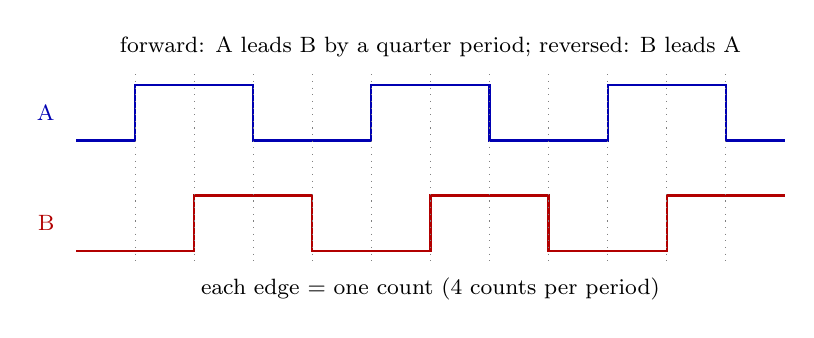
\begin{tikzpicture}[x=0.75cm,y=0.7cm]
  \draw[thick,blue!70!black] (0,0)--(1,0)--(1,1)--(3,1)--(3,0)--(5,0)--(5,1)--(7,1)--(7,0)--(9,0)--(9,1)--(11,1)--(11,0)--(12,0);
  \draw[thick,red!70!black] (0,-2)--(2,-2)--(2,-1)--(4,-1)--(4,-2)--(6,-2)--(6,-1)--(8,-1)--(8,-2)--(10,-2)--(10,-1)--(12,-1);
  \node[font=\footnotesize,anchor=east,blue!70!black] at (-0.2,0.5) {A}; \node[font=\footnotesize,anchor=east,red!70!black] at (-0.2,-1.5) {B};
  \foreach \x in {1,2,3,4,5,6,7,8,9,10,11}{\draw[dotted,gray] (\x,1.2)--(\x,-2.2);}
  \node[font=\footnotesize] at (6,1.7) {forward: A leads B by a quarter period; reversed: B leads A};
  \node[font=\footnotesize] at (6,-2.7) {each edge = one count (4 counts per period)};
\end{tikzpicture}
\captionof{figure}{Quadrature signals of an incremental encoder.}\label{fig:hw4_quad}
\end{center}
A joint also has other internal sensors: the \textbf{motor current} (which is proportional to the torque, Chapter~\ref{ch:hw6}), the \textbf{temperature} of motor and driver (to avoid burning), and the \textbf{battery voltage}. Together they are called \emph{proprioception}, the sense of one's own body. Foot robots add \textbf{force sensors} or pressure cells in the soles, which tell whether and where the foot touches the ground, important for balance.

\subsection*{The IMU}
An \textbf{IMU} (inertial measurement unit) is a small chip with
\begin{itemize}[nosep]
  \item a \textbf{3-axis accelerometer}: measures acceleration including gravity. At rest it measures $9.81\,\text{m/s}^2$ pointing upward (the force that holds it), so it tells where ``down'' is; during walking it also feels every step;
  \item a \textbf{3-axis gyroscope}: measures the angular velocity $\omega$ in rad/s or $^\circ$/s;
  \item often a \textbf{3-axis magnetometer} (compass), unreliable near motors and steel.
\end{itemize}
It is read over I2C or SPI at $100$ to $1000$ Hz (Chapter~\ref{ch:hw3}). The chip sits in the torso of the robot, and its orientation tells the robot whether it is falling. Both main sensors have a weakness:
\begin{itemize}[nosep]
  \item The \textbf{gyroscope} is smooth and fast but has a small constant \emph{bias}. To get an angle, you \emph{integrate} the angular velocity, $\theta(t)=\int\omega\,dt$, and the integral of a bias grows linearly: a bias of only $0.03$ rad/s ($1.7^\circ$/s) causes an error of $103^\circ$ after one minute. This is the \textbf{drift}.
  \item The \textbf{accelerometer} gives an absolute angle from the direction of gravity, with no drift, but it is noisy and also reacts to every acceleration of the robot (a step looks like tilt).
\end{itemize}

\section*{Sensor fusion}
The two are \emph{complementary}: the gyroscope is good at high frequencies (fast changes) and bad at low frequencies (drift); the accelerometer is the other way round. The \textbf{complementary filter} uses each in its good range: it trusts the integrated gyro in the short term and slowly pulls the result towards the accelerometer angle,
\[
\hat\theta_k=\alpha\,\big(\hat\theta_{k-1}+\omega_k\,\Delta t\big)+(1-\alpha)\,\theta^{\text{acc}}_k,\qquad \alpha\approx0.98.
\]
\begin{verbatim}
alpha = 0.98
theta = 0.0
for omega, theta_acc in zip(gyro, acc_angle):     # one pair per sample
    theta = alpha * (theta + omega * dt) + (1 - alpha) * theta_acc
\end{verbatim}
This is the low-pass filter of Chapter~\ref{ch:py7} applied to the accelerometer and a high-pass filter applied to the gyro. A simulation of a robot torso that tilts $\pm20^\circ$ at $0.3$\,Hz, with gyro bias $0.03$ rad/s and noise, an accelerometer with noise of $7^\circ$, sampled at $100$\,Hz for $10$ seconds:
\begin{center}
\includegraphics[width=0.98\textwidth]{hw/imu_fusion.png}
\captionof{figure}{Left: the raw accelerometer angle (grey, noisy) and the integrated gyro (red, drifting away). Right: the complementary filter follows the true angle (dashed).}\label{fig:hw4_fusion}
\end{center}
The RMS errors are $6.7^\circ$ for the accelerometer, $10.4^\circ$ for the gyro (and growing without bound) and $1.2^\circ$ for the filter. The time constant of the filter is $\tau=\alpha\,\Delta t/(1-\alpha)=0.49$\,s: slower disturbances are taken from the accelerometer, faster ones from the gyro. In real robots the \textbf{Kalman filter} (and its relatives, Part~\ref{part:control}) does the same job with an optimal, adaptive weighting. The principle is general: \emph{combine sensors that are wrong in different ways}.

\section*{Cameras}
A camera is a sensor that delivers a whole picture of $10^5$ to $10^7$ values at once. The simplest model is the \textbf{pinhole camera}: a point at distance $Z$ with lateral position $X$ appears on the sensor at position $x=f\,\dfrac{X}{Z}$ (Figure~\ref{fig:hw4_pin}), with the focal length $f$. Measured in pixels, $f_\text{px}=\dfrac{w/2}{\tan(\text{FOV}/2)}$: for $w=640$ pixels and a horizontal field of view of $60^\circ$ this is $554$ pixels.
\begin{center}
\begin{tikzpicture}[>={Stealth[length=2.5mm]}]
  \draw[thick] (0,-1.2)--(0,1.2) node[above,font=\footnotesize]{sensor};
  \fill (3,0) circle (0.06) node[above right,font=\footnotesize]{pinhole};
  \draw[->,gray] (-0.5,0)--(10.3,0) node[right,font=\footnotesize]{$Z$};
  \draw[very thick,orange!80!black] (9,0)--(9,1.2) node[above,font=\footnotesize,black]{object, height $X$};
  \draw[very thick,orange!80!black] (0,0)--(0,-0.6);
  \draw[thick,blue!70!black] (9,1.2)--(0,-0.6);
  \draw[<->] (0,-1.5)--(3,-1.5) node[midway,below,font=\footnotesize]{$f$};
  \draw[<->] (3,-1.5)--(9,-1.5) node[midway,below,font=\footnotesize]{$Z$};
  \node[font=\footnotesize,anchor=east] at (-0.1,-0.6) {$x$};
\end{tikzpicture}
\captionof{figure}{The pinhole model. The image of the object is upside down; by similar triangles $x/f=X/Z$. The farther the object, the smaller its image.}\label{fig:hw4_pin}
\end{center}
\textbf{Consequences.} A ball of diameter $0.13$\,m at $Z=3$\,m is $554\cdot0.13/3=24$ pixels wide, at $6$\,m only $12$ pixels. A detector needs enough pixels on the target, which sets the useful range of a camera for a given resolution. The same formula, solved for $Z$, gives the distance of an object of \emph{known size} from its pixel size: $Z=f_\text{px}\,X/x_\text{px}$ (Chapter~\ref{ch:py10} used the formula for angles). Real lenses distort images (straight lines look curved at the edges, wide-angle lenses most); \textbf{calibration} with a chessboard pattern (\texttt{cv2.calibrateCamera}) finds the focal length, the image centre and the distortion, and it is done once per camera.

\subsection*{Properties that matter}
\begin{itemize}[nosep]
  \item \textbf{Resolution and field of view:} more pixels see farther or finer; a wide field of view ($90^\circ$ and more) sees more but each object gets fewer pixels. Humanoid soccer robots need to see the ball far away \emph{and} the field lines nearby.
  \item \textbf{Frame rate} ($30$ to $120$ fps) and \textbf{latency}: a camera and USB pipeline can easily add $50$ to $100$\,ms between exposure and your program (Chapter~\ref{ch:py10}); fast motion needs the time stamp of the \emph{exposure}.
  \item \textbf{Exposure} and \textbf{motion blur:} a long exposure collects more light but blurs a moving robot or ball; indoor stadium lights flicker at $100$/$120$\,Hz, which causes banding unless the exposure is a multiple of the flicker period (\verb!v4l2-ctl --list-ctrls! shows the settings; switch off auto-exposure and fix it).
  \item \textbf{Rolling shutter:} most cheap sensors read the image row by row, in about $10$ to $30$\,ms from top to bottom. A fast rotation of the head makes vertical lines look slanted. \emph{Global shutter} cameras expose all rows at once, at a higher price.
  \item \textbf{Auto white balance} changes colours when the camera sees a lot of green: another reason to fix settings for colour-based detection.
\end{itemize}

\subsection*{Depth}
\begin{description}
  \item[Stereo camera:] two cameras at the distance $B$ (the \emph{baseline}) see a point at different positions; the shift of the point between the pictures is the \emph{disparity} $d$ in pixels, and
  \[Z=\frac{f_\text{px}\,B}{d}.\]
  With $f_\text{px}=554$ and $B=6$\,cm: $d=10$ pixels means $Z=3.3$\,m, $d=5$ means $6.7$\,m. An error of one pixel in $d$ changes the distance at $2$\,m by $\Delta Z\approx Z^2/(f_\text{px}B)=0.12$\,m: the accuracy falls with the \emph{square} of the distance.
  \item[Time of flight (ToF)] and \textbf{LiDAR} send light pulses and measure the time until the echo returns: $Z=\tfrac12 c\,t$. For $Z=3$\,m the time is $20$\,ns, so the electronics must resolve nanoseconds. A LiDAR rotates and gives a ring of distances; it is the standard sensor of mobile robots but heavy for a humanoid.
  \item[Ultrasound:] the same with sound ($340$\,m/s): cheap, but wide beam and slow.
\end{description}

\section*{Time and calibration}
Every sensor delivers its value with a delay and at its own rate. To combine the camera ($30$\,Hz, $60$\,ms late) with the IMU ($200$\,Hz, $2$\,ms late), every measurement needs a \textbf{time stamp} taken as close to the physical measurement as possible, and the clocks of all devices must agree (Chapter~\ref{ch:hw2}). In ROS~2 every message has a header with a time stamp (Part~\ref{part:ros}), and recorded data (\texttt{ros2 bag}) lets you replay and analyse a run later. Calibration, in the broad sense, includes: the zero position of every joint (the robot must know which encoder value means ``leg straight''), the gyro bias (measure it for a second while the robot stands still, then subtract it), the camera model, and the position of the sensors on the body (extrinsics, Part~\ref{part:ros}).

\begin{keyidea}[Never trust one number]
A sensor value is an \emph{estimate with an error}, not the truth. Check plausibility (is the angle within the limits? did the value jump by more than physics allows?), filter noise, detect failures (a value that never changes, or a missing time stamp), and combine independent sensors. A robot that believes a single frozen encoder will happily walk into a wall.
\end{keyidea}

\begin{example}
\textbf{Calibrating the gyro bias.} The robot stands still for $2$\,s ($200$ samples at $100$\,Hz). The mean of the gyro readings is the bias $b$; the standard deviation is the noise level $\sigma$. In Python:
\begin{verbatim}
import numpy as np
still = np.array(gyro_samples[:200])
bias, sigma = still.mean(), still.std(ddof=1)
corrected = np.array(gyro_samples) - bias
\end{verbatim}
With $b=0.03$ rad/s and $\sigma=0.02$ rad/s the uncertainty of the bias estimate is only $\sigma/\sqrt{200}=0.0014$ rad/s (Chapter~\ref{ch:stats}), twenty times smaller than the bias: the drift after one minute falls from $103^\circ$ to $5^\circ$. Bias changes with temperature, so repeat the calibration whenever the robot has been switched on and is standing still.
\end{example}

\section*{Practice problems}
\begin{enumerate}[label=\textbf{\thechapter.\arabic*}]
  \item Explain the difference between accuracy and precision. Which one can you improve by calibration, which by averaging?
  \item A $14$-bit ADC measures $\pm2$\,g (range of $4$\,g). What is the resolution in mg per count?
  \item An encoder has $2048$ lines per turn and is read in quadrature. How many counts per turn, and what angle is one count? The motor is connected to the joint by a $1\!:\!10$ gear. What is the angle resolution of the joint, and how many counts for a joint movement of $90^\circ$?
  \item A signal contains a $60$\,Hz vibration. At which sample rates is it measured without aliasing, and what do you see when you sample at $80$\,Hz?
  \item A gyro with bias $0.5^\circ$/s is integrated for $2$ minutes. How large is the angle error? How do you reduce it?
  \item Why can the accelerometer alone not give the tilt of a walking robot, and why can the gyro alone not give it for long?
  \item In the complementary filter with $\alpha=0.98$ and $\Delta t=0.01$\,s, compute the time constant. What happens for $\alpha=0.999$ and for $\alpha=0.5$?
  \item A camera with $1280$ pixels width and $90^\circ$ horizontal field of view looks at a $0.13$\,m ball. Compute $f_\text{px}$ and the width of the ball in pixels at $2$, $5$ and $10$\,m.
  \item A stereo camera with $f_\text{px}=700$ and baseline $B=12$\,cm measures a disparity of $14$ pixels. How far is the object? How large is the distance error for a disparity error of $0.5$ pixels?
  \item[\textbf{\thechapter.10}$\star$] Write a program that simulates a gyro with bias and noise and an accelerometer with noise (as in Figure~\ref{fig:hw4_fusion}) and compares the RMS error of the complementary filter for $\alpha=0.9,0.98,0.998$. Which one is best, and why is there an optimum?
\end{enumerate}
